\chapter{Dispersion}
\label{ch:Dispersion}
In the context of optics, "Dispersion" refers to the fact that the speed of light waves in materials such as glass depends on the temporal frequency of those waves. If a beam of light containing multiple different temporal frequencies enters a block of glass at an angle, the constituent frequencies will disperse spatially according to Snell's Law~\cite{Snell}. If a laser pulse with a certain duration consisting of a range of temporal frequencies enters the same block of glass at a right angle, a longer pulse may exit in the other end because the different frequencies of light have taken different amounts of time to propagate through it. This chapter explains how the impact of dispersion on laser pulses can be understood from first principles. 

\section{Pulses and spatial frequency}
Consider Eq.~\ref{eq:pulse} under the assumption that the pulse is propagating in a spatially homogeneous medium, so that $\betag(z,\omega)=\betag(\omega)$,

\begin{align}
\label{eq:spatially_uniform}
    \E(z,t) &= \frac{1}{2\pi}\int_{-\infty}^{\infty} \Tilde{\E}(z,\omega) e^{i\betag(\omega)z-i\omega t} d\omega.
\end{align}
In a bulk medium, $\betag(\omega)=n(\omega)\omega/c$, where $n(\omega)$ is the refractive index of the material and $c$ is the speed of light. For a waveguide such as an optical fiber, $\betag(\omega)$ must be determined by solving Maxwell's equations as explained in this \href{https://youtu.be/z7fyT3etgis}{video tutorial}. Additionally, the durations of the envelopes of pulses considered in this primer are assumed to be much longer than the duration of a single oscillation at their carrier frequencies, $\omega_0/2\pi\approx 200$~THz as illustrated in Fig.~\ref{fig:bandwidth} a). 

\begin{figure}
    \centering
    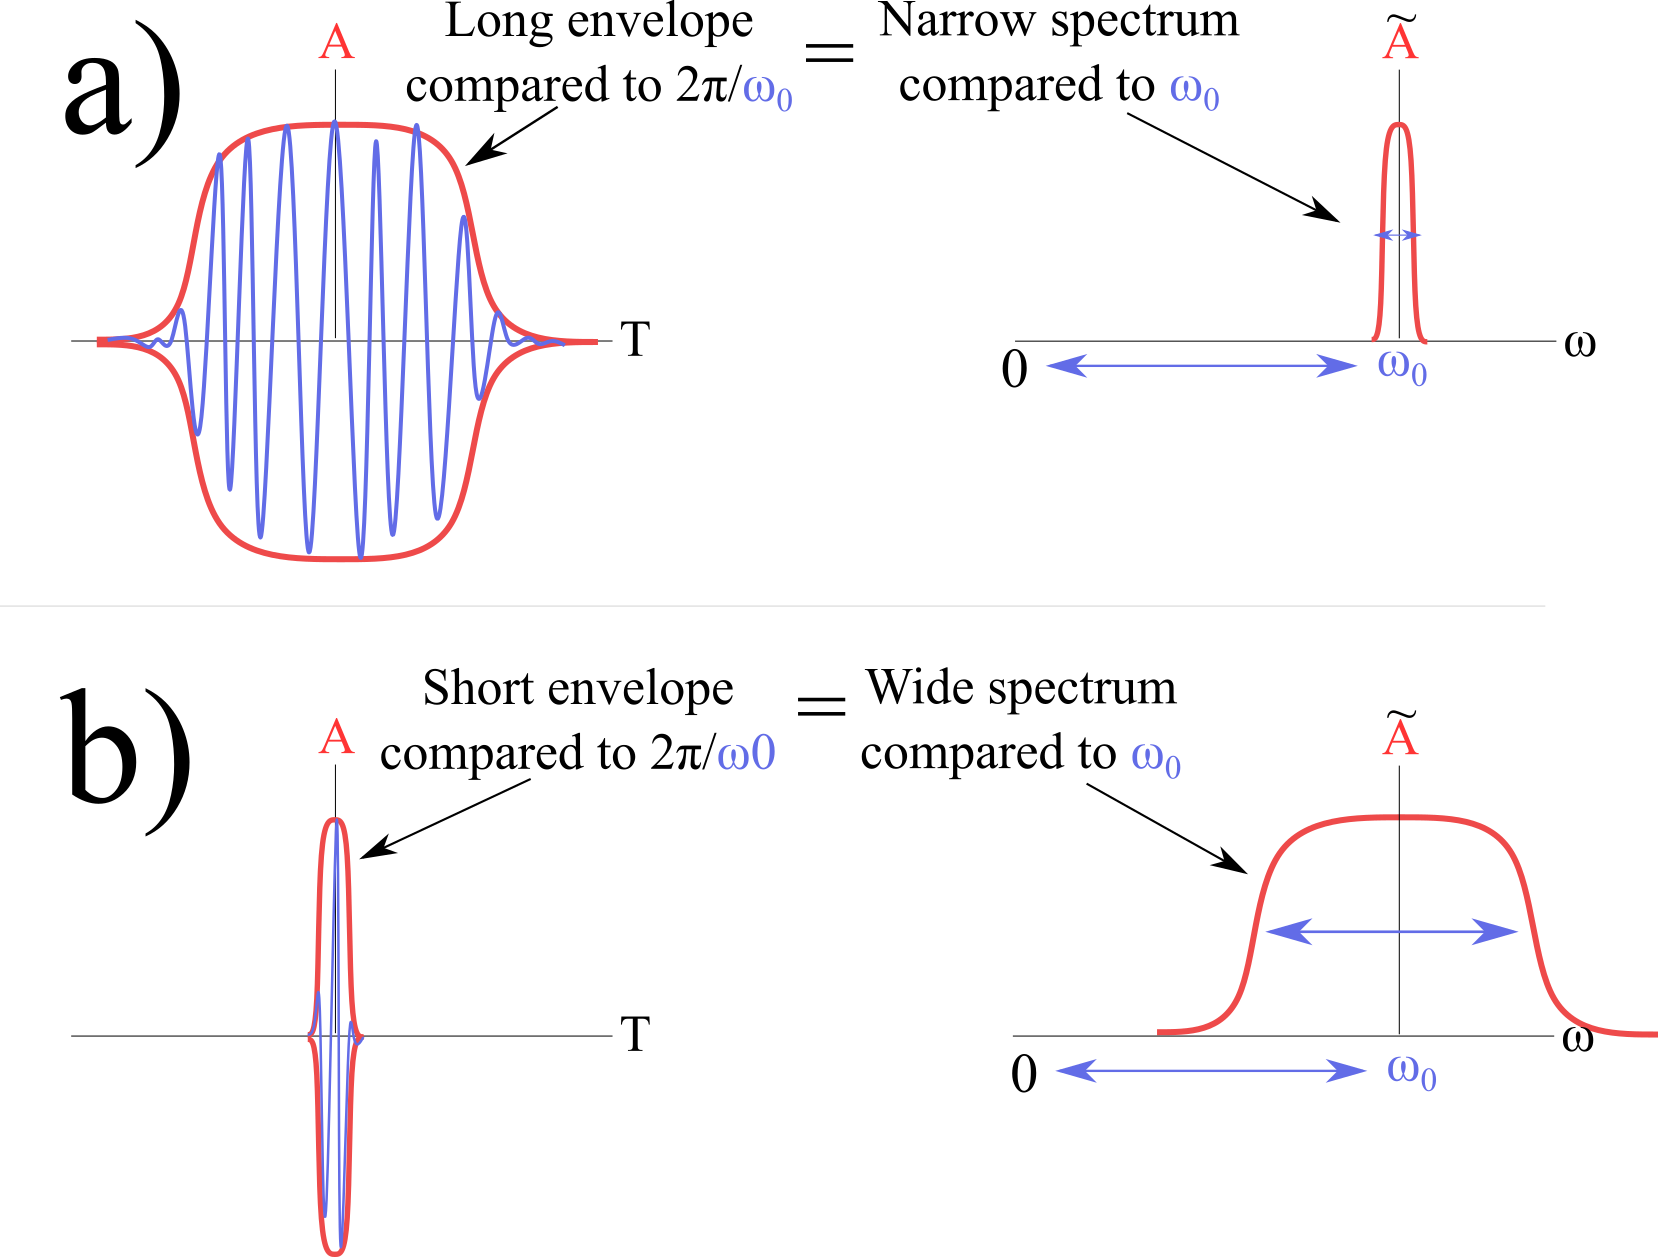
\includegraphics[width=1\linewidth]{figures/bandwidth.png}
    \caption{a) A pulse with a long duration compared to the duration of a single electric field oscillation at the carrier frequency will have a narrow spectrum. b) Conversely, a short pulse will have a wide spectrum.}
    \label{fig:bandwidth}
\end{figure}

Under these assumptions, the spectral width of the pulse is so narrow that $\betag(\omega)$ can be Taylor-approximated around the carrier frequency as
\begin{align}
\label{eq:beta_approx}
    \betag(\omega)&\approx \betag(\omega_0)+\partial_\omega\betag|_{\omega_0}(\omega-\omega_0)+\frac{1}{2!}\partial^2_\omega\betag|_{\omega_0}(\omega-\omega_0)^2+
    \frac{1}{3!}\partial^3_\omega\betag|_{\omega_0}(\omega-\omega_0)^3+... \\ \nonumber
    &= \sum_{n=0}^{\infty} \frac{1}{n!}\partial^n_\omega\betag|_{\omega_0}(\omega-\omega_0)^n\\ \nonumber
    &=\sum_{n=0}^{\infty} \frac{1}{n!}\betag_n(\omega-\omega_0)^n.
\end{align}
With this simplification in mind, the expression for a pulse propagating through a medium becomes
\begin{align}
\label{eq:beta_approx_applied}
    \E(z,t) &= \frac{1}{2\pi}\int_{-\infty}^{\infty} \Tilde{\E}(z,\omega) e^{i(\betag_0+\betag_1(\omega-\omega_0)+\frac{1}{2}\betag_2(\omega-\omega_0)^2+...)z-i\omega t} d\omega.
\end{align}


\section{$\betag_0$ - How much the carrier gets delayed}
Because the term containing $\betag_0$ does not depend on $\omega$, it can be moved outside the integral in Eq.~\ref{eq:beta_approx_applied}. Multiplying by $1=\exp(-i\omega_0t)\exp(i\omega_0t)$ yields
\begin{align}
\label{eq:beta_approx_applied}
    \E(z,t) &= \frac{1}{2\pi} e^{i\betag_0z-i\omega_0t}  \int_{-\infty}^{\infty} \Tilde{\E}(z,\omega) e^{i(\betag_1(\omega-\omega_0)+\frac{1}{2}\betag_2(\omega-\omega_0)^2+...)z-i(\omega-\omega_0) t} d\omega.
\end{align}
The exponential outside the integral implies that if one observes the complex electric field in the medium over a duration consisting of a few cycles of the carrier, it will look like a complex plane wave with a temporal frequency of $\omega_0$ and a spatial frequency of $\betag_0$. See \href{https://www.desmos.com/calculator/ausd1wnl2j}{this interactive graph} for an illustration of the impact of $\betag_0$ on the propagation of a real plane wave in a medium. 

\subsection{Phase velocity}
\label{sec:Phase_velocity}
The carrier wave will peak when $\betag_0z-\omega_0t$ is an integer multiple of $2\pi$. Consider for simplicity the peak corresponding to $\betag_0z-\omega_0t=0$. If time advances by $0<\Delta t$, the original value of $z$ does not satisfy $\betag_0z-\omega_0(t+\Delta t)=0$. Instead, the peak will be at some new location $z+\Delta z$, where
\begin{align}
    \betag_0(z+\Delta z)-\omega_0(t+\Delta t)=0\\ \nonumber
    \betag_0\Delta z-\omega_0\Delta t=0.
\end{align}
Since the peak has shifted by $\Delta z$ during the time $\Delta t$, one can define the "phase velocity" (or alternatively the "carrier velocity") as
\begin{align}
\label{eq:Phase_velocity}
    v_p &= \frac{\Delta z}{\Delta t} = \frac{\omega_0}{\betag_0}.
\end{align}


\section{$\betag_1$ - How much the envelope of a pulse centered at the carrier gets delayed}
The integral in Eq.~\ref{eq:beta_approx_applied} represents the envelope of the complex electric field propagating through the medium. Rearranging the exponential terms, one obtains
\begin{align}
\label{eq:envelope_beta1}
    \E(z,t) &= \frac{1}{2\pi} e^{i\betag_0z-i\omega_0t}  \int_{-\infty}^{\infty} \Tilde{\E}(z,\omega) e^{i\betag_1(\omega-\omega_0)z-i(\omega-\omega_0) t} e^{i(\frac{1}{2}\betag_2(\omega-\omega_0)^2+...)z} d\omega.
\end{align}
Applying the same analysis behind Eq.~\ref{eq:Phase_velocity}, one finds that the peak of the envelope of the complex electric field propagates at the so-called "group velocity" (or alternatively the "envelope velocity") given by
\begin{align}
\label{eq:group_velocity}
    v_g &= \frac{(\omega-\omega_0)}{\betag_1\cdot(\omega-\omega_0)} = \frac{1}{\betag_1} = \frac{1}{\partial_\omega\betag}.
\end{align}
See \href{https://www.desmos.com/calculator/rq2physwac}{this interactive graph} for an illustration of the difference between phase- and group velocity. Note that Eq.~\ref{eq:group_velocity} agrees with the prediction of Eq.~\ref{eq:delay_definition} that a large, positive change in the phase w.r.t. $\omega$ should lead to a large delay.




\section{$\betag_2$ - How much the frequencies constituting the envelope of a pulse centered at the carrier get delayed relative to each other}
\label{sec:GVD}
Applying Eq.~\ref{eq:envelope} to Eq.~\ref{eq:envelope_beta1} allows one to "factor out" the fast but predictable spatial and temporal oscillations of the carrier and focus on the envelope:
\begin{align}
    \A(z,t)  &= \frac{1}{2\pi}  \int_{-\infty}^{\infty} \Tilde{\A}(z,\omega) e^{i\betag_1(\omega-\omega_0)z-i(\omega-\omega_0) t} e^{i(\frac{1}{2}\betag_2(\omega-\omega_0)^2+...)z} d\omega.
\end{align}
To simplify further, one can define $T=t-\betag_1z$, which is the "time relative to the moment at which the envelope of the pulse arrives at a distance $z$". Using $T$ instead of $t$ is convenient because many optics experiments involve sending pulses of light through a medium with a fixed length and tracking the measured power over time after the light leaves the medium:   
\begin{align}
    \A(z,T)  &= \frac{1}{2\pi}  \int_{-\infty}^{\infty} \Tilde{\A}(z,\omega) e^{i\betag_1(\omega-\omega_0)z-i(\omega-\omega_0) (T+\betag_1z)} e^{i(\frac{1}{2}\betag_2(\omega-\omega_0)^2+...)z} d\omega \\ \nonumber
    &= \frac{1}{2\pi}  \int_{-\infty}^{\infty} \Tilde{\A}(z,\omega) e^{i(\frac{1}{2}\betag_2(\omega-\omega_0)^2+...)z-i(\omega-\omega_0)T} d\omega.
\end{align} 
As explained via Eq.~\ref{eq:spectrum_time_example}, a positive(negative) value of $\betag_2$ implies that lower(higher) temporal frequencies propagate faster than higher(lower) temporal frequencies, causing the envelope of the pulse to broaden in the time domain. Alternatively, one can consider Eq.~\ref{eq:GNLSE} with only the $\betag_2$ term,
\begin{align}
    \label{eq:heat_equation}
    \partial_z \A = -i  \frac{\betag_2}{2}\partial_T^2\A,
\end{align}
which is identical to the so-called "Heat Equation"~\cite{Fourier_heat_original,Fourier_heat_english}. See also 
\href{https://digitalcommons.ursinus.edu/cgi/viewcontent.cgi?article=1008&context=triumphs_differ}{this tutorial}. To obtain $\A(z,T)$ given $\A(z=0,T)$ and thus $\tilde{\A}(z=0,\omega)$, first compute the Fourier Transform of Eq.~\ref{eq:heat_equation} to obtain
\begin{align}
    \label{eq:beta2_broadening}
    \partial_z \Tilde{\A} &= -i  \frac{\betag_2}{2} (i(\omega-\omega_0))^2 \Tilde{\A} \\ \nonumber
    &= i  \frac{\betag_2}{2}(\omega-\omega_0)^2\Tilde{\A} \\ \nonumber
    \Tilde{\A}(z,\omega)&=\Tilde{\A}(0,\omega)e^{i\frac{\betag_2}{2}(\omega-\omega_0)^2z} \\ \nonumber
    \A(z,T) &= \IFT\left\{  \Tilde{\A}(z,\omega)   \right\}.
\end{align}
For a Gaussian pulse, Eq.~\ref{eq:beta2_broadening} can be solved \href{https://drive.google.com/file/d/17Ab3bg0Hx0x8J-5lR29ejFg0eOlv6Psh/view?usp=sharing}{analytically}. The result indeed implies that the pulse will broaden temporally, while Eq.~\ref{eq:chirp_definition} applied to the result confirms that $\betag_2>0$ implies that lower frequencies will arrive earlier than higher frequencies. Because the magnitude of the phase shift caused by $\betag_2$ grows quadratically with the distance between a given frequency component and the carrier, shorter pulses with greater spectral widths will temporally broaden more over the same distance than shorter ones with smaller bandwidths. A characteristic length over which the broadening due to $\betag_2$ becomes significant can be defined as
\begin{align}
    \label{eq:Dispersion_length}
    L_{2} &= \frac{T_0^2}{|\betag_2|}.
\end{align}
See \href{https://www.youtube.com/watch?v=BP6Ra98AEuU}{this video} for an illustration of the impact of dispersion on a Gaussian pulse. 

\subsection{The "Zero Dispersion Frequency"}
\label{subsec:ZDF}
For a given medium where $\betag(\omega)$ is known, one can compute the value of $\betag_2$ near a given carrier frequency, $\omega_0$, as
\begin{align}
\label{eq:ZDF}
    \betag_2(\omega) &= \betag_2|_{\omega=\omega_0} + \betag_3|_{\omega=\omega_0}\cdot(\omega-\omega_0)+\frac{1}{2}\betag_4|_{\omega=\omega_0}\cdot(\omega-\omega_0)^2 +...,
\end{align}
which allows one to solve for the specific frequency (or \emph{frequencies}, plural!), $\omega_{ZD}$, where $\betag_2(\omega_{ZD})=0$. This "Zero Dispersion Frequency" is important because a number of nonlinear mechanisms are more efficient for frequencies at $\omega_{ZD}$ or ones close to it where $\betag_2<0$. Therefore, determining the value(s) of $\omega_{ZD}$ for a given medium is crucial when conducting experiments in nonlinear optics. The zero dispersion frequency of a particular fiber can be measured experimentally using commonly available optical laboratory equipment~\cite{zero_disp_measurement}.
Historically, optical fibers for telecommunication were designed so that $\betag_2\approx0$ close to near-infrared frequencies of laser light ($\approx$190-230~THz $\approx$1310-1550~nm) that were easy to generate, modulate and detect. The intention was to prevent temporal broadening and thus overlap and interference of pulses carrying digital information. Since the mid 2000's, advancements in electronic dispersion compensation have rendered such fiber designs obsolete and even deleterious, as nonlinear effects that distort signals by altering their phases and amplitudes are more significant close to $\omega_{ZD}$.


\section{$\betag_n$ - Higher order delays}
Having understood that the slope of $\betag(\omega)$ (i.e. $\betag_1$) determines the propagation speed of the pulse envelope while the curvature of $\betag(\omega)$ (i.e. $\betag_2$) determines the temporal broadening of the pulse, these insights can be generalized. For example, $\betag_3>0$ implies that the term $i\betag_3/6(\omega-\omega_0)^3z$ causes a positive $\partial_\omega\phi$ for all frequencies except the carrier. Thus, both the higher and lower frequencies contributing to the pulse will begin to trail behind the main pulse, leading to asymmetric temporal broadening. Furthermore, $\betag_4>0$ implies that $i\betag_4/24(\omega-\omega_0)^4z$ causes additional symmetric temporal broadening on top of what is caused by $\betag_2$. See Fig.~\ref{fig:dispersion_combined} for an illustration of the impact of different $\betag_n$ terms on the temporal profile of a Gaussian pulse. How many terms in the expansion of $\betag(\omega)$ to include when analyzing the evolution of a pulse propagating through a medium depends on the spectral width of the pulse, which is inversely proportional to its duration. For pulses above 1~ps, orders higher than $\betag_3$ rarely contribute much. In numerical simulations of supercontinuum generation with pulses with a duration on the scale of 10~fs, orders up to $\betag_8$ are often included for good measure. Similarly to Eq.~\ref{eq:Dispersion_length}, the characteristic lengths over which higher order dispersion effects become significant are defined by
\begin{align}
\label{eq:dispersion_length_general}
    L_{n} &= \frac{T_0^n}{|\betag_n|}.
\end{align}
See \href{https://www.youtube.com/watch?v=E3S0BQiy3p8&ab_channel=YourFavouriteTA}{this video tutorial} for further details on dispersion.

\begin{figure}
    \centering
    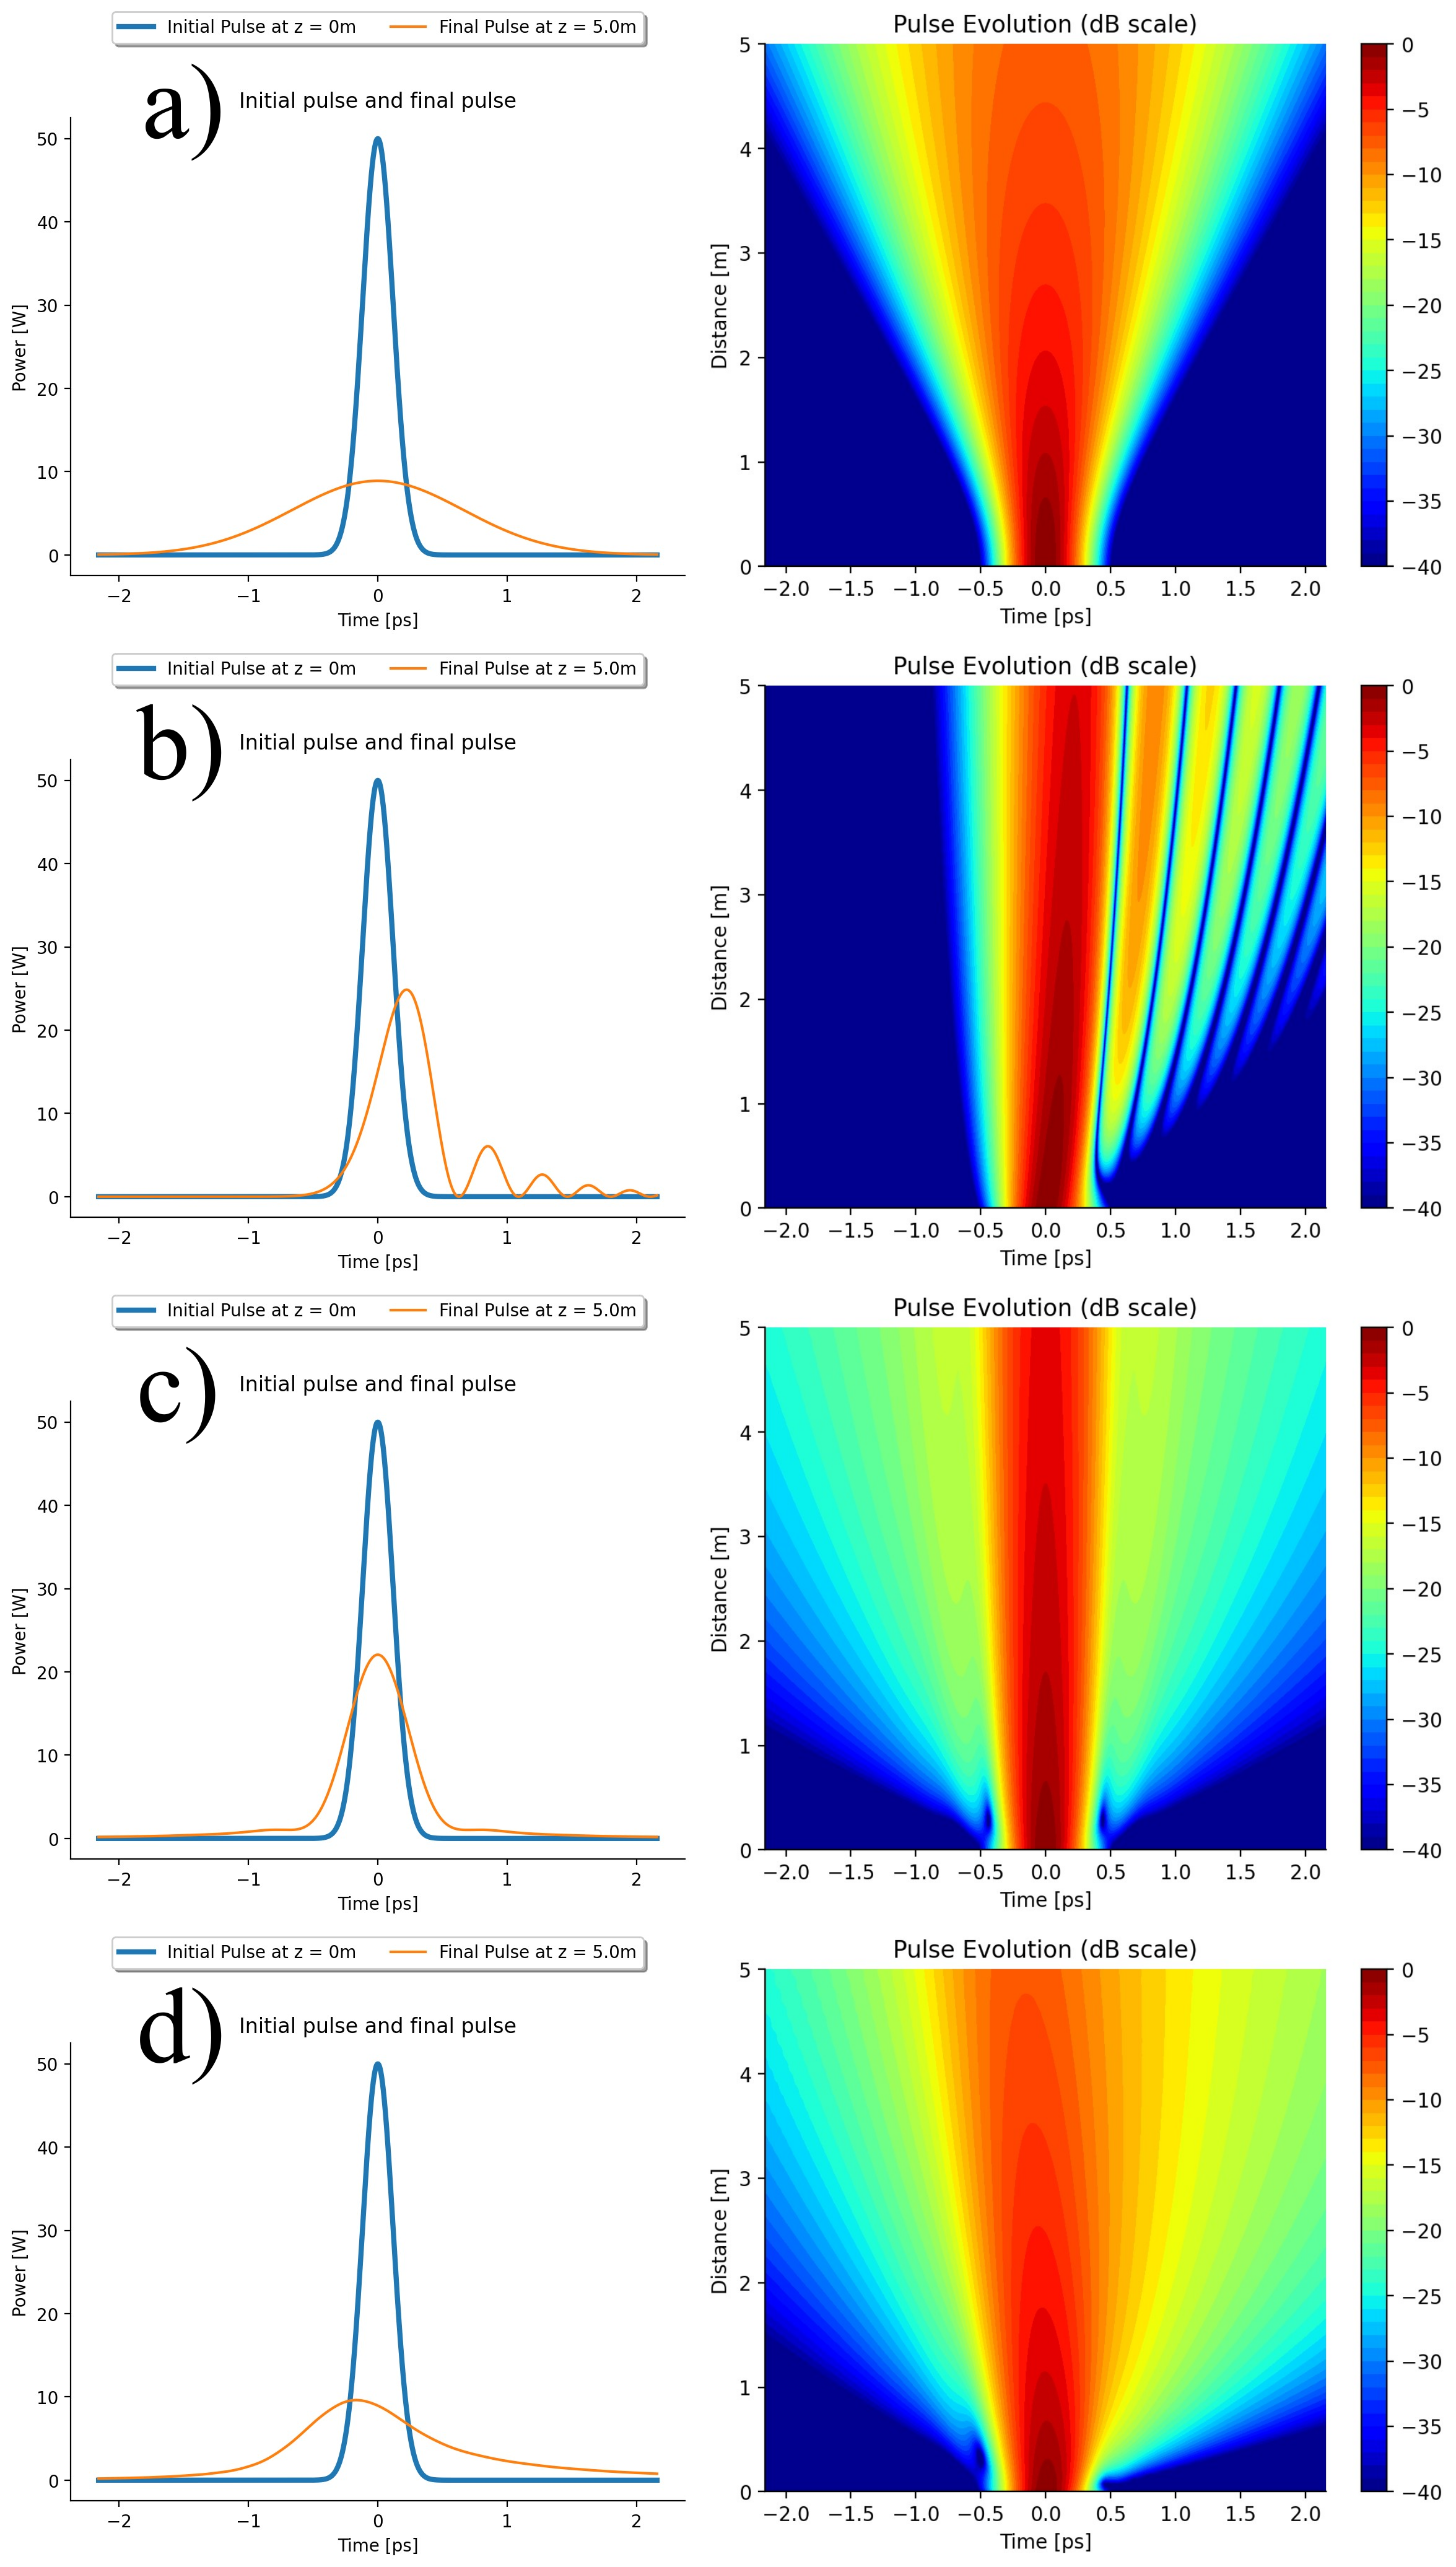
\includegraphics[width=0.75\linewidth]{figures/dispersion_combined.png}
    \caption{Illustration of the effect of different $\betag_n$ terms on a Gaussian pulse in the time domain. Left column shows a comparison of the power envelope of the pulse before and after propagating through media with different $\betag_n$ terms. Right column shows the evolution of the power envelope with distance. a) Medium with $\betag_2<0$. b) Medium with $\betag_3>0$. c) Medium with $\betag_4<0$. d) Medium where $\betag_2<0$, $\betag_3>0$ and $\betag_4<0$ are present simultaneously. 
    Figures generated using the numerical simulation in \href{https://colab.research.google.com/drive/1PW9smFA3PECvcXyWpZcW1ogY4W3hEYFt?usp=sharing}{this interactive notebook}, which the reader is encouraged to experiment with.}
    \label{fig:dispersion_combined}
\end{figure}

\section{Are $\alpha(\omega)$ and $\betag(\omega)$ independent?}
\label{sec:KK_relations}

In Eq.~\ref{eq:GNLSE}, $\alpha$ is treated as a constant because its frequency dependence is usually weak across the bandwidth of a typical pulse. However, one could in principle include a Taylor expansion of $\alpha(\omega)$ as was done with $\betag(\omega)$. Interestingly, it turns our that the functions $\alpha(\omega)$ and $\betag(\omega)$ for a given medium are related through the so-called \href{https://en.wikipedia.org/wiki/Kramers%E2%80%93Kronig_relations#Related_proof_from_the_time_domain}{Kramers-Kronig Relations} and that knowing one enables the calculation of the other. As a consequence, $\alpha(\omega)$ and $\betag(\omega)$ \emph{cannot} be chosen independently. Proving the connection mathematically is tricky, but physically, the intuition is that the frequency dependent absorption  of $\alpha(\omega)$ fundamentally is exactly what gives rise to frequency dependent phase delay, $\betag(\omega)$. Additionally, the response of the medium at a given location to an applied electric field can only depend on \emph{the current and past} values of the electric field at that location for causality to be respected, which further constrains what combinations of attenuation and phase delay are allowed. Conveniently, it turns out that if $\alpha(\omega)=\alpha$ is treated as a constant w.r.t. frequency, its value can be changed freely without impacting any of the values of $\betag_n$.  

Please see \href{https://www.youtube.com/watch?v=vzBnsG2rKWs}{this video } and \href{https://www.youtube.com/watch?v=rFTUTxPHYYw}{this other video} for more details on the Kramers-Kronig Relations. See \href{https://www.desmos.com/calculator/1zymtgbbrv}{this interactive graph} for a tutorial on using causality and the Kramers-Kronig Relations in the time domain to relate $\alpha(\omega)$ to $\betag(\omega)$.

